\chapter{A Two Step Bayesian Model for Matching Cell Line and Patient Genomic Profiles}
\label{ch:cell_line_patients}
\index{Instructions for Preparing Dissertations, Theses, and Reports%
@\emph{Instructions for Preparing Dissertations, Theses, and Reports}}%

\section{Introduction}
\label{sec:intro}

In a precision medicine paradigm, the patient's specific genetic architecture is assessed to propose a personalized treatment that is expected to be optimal for that individual. In this context, there is a trend in modern medicine to move from generalized treatment approaches towards the tailored treatment strategy that is dictated by their genomics or molecular profile. This paradigm shift accelerates the needs for advances in pharmacogenomics technology and associated analytical methods. In this paper, we develop methods to meet this demand, inclduing in particular novel priors for random structures. Briefly, we propose  developing an integrative statistical framework, that merge  multiplatform genomics ('omics, in short) profiles from multiple model systems (e.g. patients and cell-lines) for finding significant drug targets, pre-clinical models for appropriate drug discovery and repurposing  and, finally, to calibrate therapeutic potential for future patients. By identifying these similarities (and differences) across model systems, we are able to gather more refined information about the patient than what is contained in their specific profile, while still proposing a personalized treatment that is strongly tied to the patient's profile - through appropriate integration of various data sources. 

The objective of this paper is then to construct a novel Bayesian statistical  approach for  matching patient gene profiles with cell line profiles. Such inference is needed, among many other applications, for data integration, precision medicine and patient specific treatment assignment. The expansion of modern medicine and fast growth of research in health sciences  have  led to a great increase in available  data on multiple sources/platforms such as The Cancer Genome Atlas (TCGA, \url{tcga-data.nci.nih.gov}), Cancer Cell Line Encyclopedia (CCLE, \url{portals.broadinstitute.org/ccle}), International Cancer Genome Consortium (ICGC, \url{icgc.org}) to name a few.  A model-based approach  for matching of a patient profile with data from other sources, such as from cell lines, allows us to access a  wider range of information to predict a patient’s response to specific treatments. Important for the envisioned application, the matching should be carried out on the basis of a biologically meaningful signal only, putting aside mere noise.

A cell line is a culture of cells extracted from a tissue (e.g.,
cancer cells from a tumor in a human tissue) and grown in an in-vitro
environment that simulates the environment of the tissue in the
organism where it was extracted. Therefore, cell lines serve as
models to study cancer biology.  Information  from the response to a
drug or treatment applied to cell lines (cultivated {\it in-vitro}) is used
to infer about the  expected response {\it in vivo}
\citep{goodspeed2016}. Similarly, individuals can be grouped
according to similarities between their profiles and observed profiles
in a fixed set of cell lines.
 In such scenarios,  the mapping of
cell lines and patients  opens the possibility to construct treatment
recommendations 
based on results for the corresponding cell lines \citep{sinha2015}. We propose a statistical  approach that seamlessly  combines the
output of the Bayesian mixture model
 based on a proposal by \cite{poe_2002} with a novel two-way Bayesian non-parametric (BNP) mixture model  that is constructed as an extension of a  BNP bi-clustering model of \cite{lee2013}. 

\cite{poe_2002} propose a Gaussian-uniform mixture model for probability of expression
 (POE). Later in the model construction we shall use the latent trinary signal of the POE model to carry out nested clustering of patient samples and the desired matching with cell lines. The uniform component in the POE models havier tails associated with genes that are over- and under-expressed, while the Gaussian term corresponds to regularly expressed genes. The authors argue that, by trichotomizing  gene expressions into these 3 categorical levels, the POE approach smoothly removes uninformative biological and instrumental noise that is naturally present in genomic profile data, therefore strengthening downstream  analysis.

The clustering of patient samples and the desired match with cell lines builds on a model developed of \cite{lee2013}, who present a Bayesian model  (NoB-LoC)  that identifies genes (columns) that are relevant for clustering of samples/individuals (rows).  The identified genes are then partitioned  in such a way that genes within the same subgroup (column-wise clusters)  give rise to a common nested partition of individuals (row-wise clusters). 
 The approach is motivated by the observation that high-dimensional protein profiles make it hard to find meaningful
clusters of samples/individuals. Researchers therefore often restrict attention to groups of proteins that are
expected to lead to more meaningful and interpretable results. NoB-LoC identies such groups in a seamless process, together with the nested clustering of samples. The NoB-LoC model conveniently allows for different clustering of samples with respect to different groups of proteins. In our context, this translates to association of cell lines and patients depending on the set of proteins in the profile.



Developing the outlined model consturction, this chapter makes two major contributions: the first one is the  integration of POE with the two-way clustering building on the NoB-LoC model. The second, and perhaps more important contribution is the extension of the NoB-LoC model to allow for explicit probabilistic matching of profiles that could come from distinct sources (e.g., cell
lines and patients). In short,  in the proposed approach we first use the NoB-LoC model to partition the proteins 
according to a zero enriched P\'olyia urn process where some proteins are set aside as inactive proteins, while the selected proteins are grouped into protein clusters (active proteins). Within each protein cluster, the samples are partitioned again, using a partition model that matches patients to cell lines. The motivation is that the usually high-dimension protein profiles make it hard to find similar samples to be clustered together, therefore restricting the attention to groups of proteins is expected to lead to more meaningful and interpretable results. This procedure also naturally allows for identification of co-expressed proteins in the form of protein clusters, i.e. a group of genes that are biologically correlated are also expected to have their expression levels "tied together" along different samples. Finally, the NoB-LoC model conveniently allows for different clustering of samples depending on the subsample of proteins that is considered. In our problem, this translates to association of cell lines and patients depending on the set of proteins in the profile.

The real data used in the statistical analysis comes from an experiment using reverse phase protein arrays (RPPA)
which record the expression of selected proteins simultaneously on multiple cell lines and patients samples \citep{rppa_ref}. The dataset analyzed here consists of lung cancer protein expressions (233 proteins) measured in 687 patients and 124 cell lines. Data is batch corrected, i.e., they are also adjusted for the batch effect difference between cell line and patients' data).

\section{ POE Model}
\label{sec:poe}

In this section we describe the POE (probability of expression) model defined in \cite{poe_2002}. We modified some of the priors in order to obtain analytical full-conditionals for as many parameters as possible, which facilitates the MCMC implementation in the larger, encompassing model (more details ahead and also in appendix \ref{sec:full_cond}).

Each observation $y_{sg}$ consists of expression levels for protein (gene) $g\in \{1, \dots, G\}$ and sample $s \in \{1, \dots, S\}$. Latent variables $e_{sg}$ indicate high expression of gene $g$ in sample $t$ ($e_{sg} = 1$), normal expression ($e_{sg} = 0$) and under expression ($e_{sg} = -1$). Each possible value of $e_{sg}$ determines a different distribution for the observed gene expressions according to the following Gaussian-Uniform mixture model

$$(y_{sg} \mid e_{sg}) \sim \begin{cases}
Unif(\alpha_s + \mu_g, \ \alpha_s + \mu_g + k^+_g), &\mbox{ if } e_{sg} = 1,\\
N(\alpha_s + \mu_g, \ \sigma^2_g), &\mbox{ if } e_{sg} = 0,\\
Unif(\alpha_s + \mu_g - k^-_g, \ \alpha_s + \mu_g), &\mbox{ if } e_{sg} = -1.
\end{cases}$$\\

The lengths  $k^+_g$ and $k^-_g$ of the support of the uniform components should cover the tails of the corresponding gene expression distribution implying heavier tails than the Gaussian distribution. Under normality, the great majority of the samples (probability 0.997) concentrate within 3 standard deviations from the mean; therefore the constraints $k^+_g > k_0 \sigma_g, \ k^-_g > k_0 \sigma_g$ imply heavier than Gaussian tails for fixed values of $k_0$ greater than, say, 3. 

We now define the weights for each term in the mixture by the probability vectors $\bfpi_g:=(\pi^-_g, \pi^0_g, \pi^+_g), \ g \in \{1, \dots, G\}$ where $\pi^+_g = P(e_{sg} = 1 \mid \bfpi_g) $, $\pi^0_g = P(e_{sg} = 0 \mid \bfpi_g)$ and $\pi^-_g = P(e_{sg} = -1 \mid \bfpi_g).$ We assume $(\bfpi_g \mid \bfeta_{\pi}) \sim Dirichlet(\bfeta_{\pi}).$

Figure \ref{fig:poe_ex} illustrates the implied mixture model in the context of density estimation. The augmentation of the parameter space with inclusion of indicatior variables  $e_{st}$ allows for identification of up- and down-regulated genes that are not well captured bythe light tails of a single Gaussian component.

\begin{figure}[!ht]
  \centering
  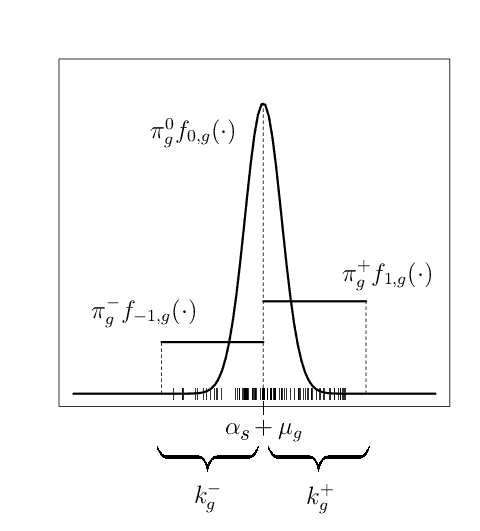
\includegraphics[scale = 0.5]{./veera/ex_poe_a_mod.png}
  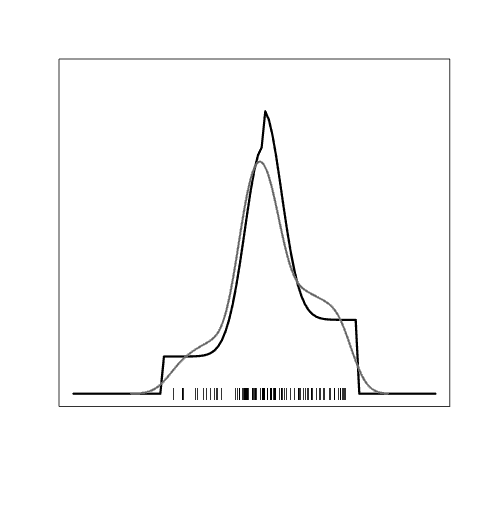
\includegraphics[scale = 0.5]{./veera/ex_poe_b.png}
\caption{Left panel: Weighted components of the Gaussian-Uniform mixture model. Right panel: density estimates using Gaussian-Uniform mixture (black line) and using kernel estimate (gray line). Vertical bars represent data generated from the Gaussian-Uniform mixture.}
\label{fig:poe_ex}
\end{figure}


Posterior probabilities of differential expression are determined by Bayes rule as 
\begin{align}
p^+_{sg} &:= P(e_{sg} = 1 \mid y_{sg}, \bfpi_g, f_{1,g}, f_{0,g}) \nonumber \\
&=\frac{\pi^+_g f_{1,g}(y_{sg})}{ \pi^+_g f_{1,g}(y_{sg}) + \pi^0_g f_{0,g}(y_{sg}) + \pi^-_g f_{1,g}(y_{sg})}\times \mathds{1}(y_{sg} \in S_{f_{1,g}}) \nonumber \\
&=\frac{\pi^+_g f_{1,g}(y_{sg})}{ \pi^+_g f_{1,g}(y_{sg}) + \pi^0_g f_{0,g}(y_{sg})}\times \mathds{1}(y_{sg} \in S_{f_{1,g}}), 
\label{eq:p+}
\end{align}

\noindent where $\mathds{1}(\cdot)$ is the indicator function and $S_{f_{1,g}}$ denotes the support of $f_{1,g}$. Analogously,

\begin{align}
p^-_{sg} :&= P(e_{sg} = -1 \mid y_{sg}, \bfpi_g, f_{-1,g}, f_{0,g}) \nonumber\\
&=\frac{\pi^-_g f_{-1,g}(y_{sg})}{ \pi^-_g f_{-1,g}(y_{sg}) + \pi^0_g f_{0,g}(y_{sg})}\times \mathds{1}(y_{sg} \in S_{f_{-1,g}}).
\label{eq:p-}
\end{align}

Equations \eqref{eq:p+} and \eqref{eq:p-} are used for visualization of sample specific gene profiles. Since $p^+_{sg}$ and $p^-_{sg}$ are not simultaneously positive, the differences $d_{sg}:=p^+_{sg} - p^-_{sg}$ will fall in the interval $[-1,1]$, therefore serving as a unidimensional measure of gene expression ( $d_{sg}\approx 1$ for highly expressed and $d_{sg}\approx -1$ for underexpressed genes).

The model is completed by the prior specification $(\mu_g \mid \theta_{\mu}, \tau_{\mu}) \sim N(\theta_{\mu}, \tau_{\mu}), $
$(\alpha_s \mid \mu_{\alpha}, \tau_{\alpha}) \sim N(\mu_{\alpha}, \tau_{\alpha}) \mbox{ restricted to } \sum^S_{s=1} \alpha_s = 0,$
$(\sigma^2_g \mid \gamma, \lambda) \sim InvGamma(\gamma, \lambda),$
$(k^+_g \mid \alpha_{k^+}, \beta_{k^+}) \sim InvGamma(\alpha_{k^+}, \beta_{k^+}),$
$(k^-_g \mid \alpha_{k^-}, \beta_{k^-}) \sim InvGamma(\alpha_{k^-}, \beta_{k^-}).$ We also chose prior models for hyperparameters as $\theta_{\mu} \sim N(m_{\mu}, s^2_{\mu})$,
$\tau_{\mu} \sim InvGamma(a_{\tau_{\mu}}, b_{\tau_{\mu}})$,
$\alpha_{k^+} \sim Exp(\lambda_{\alpha_{k^+}})$,
$\alpha_{k^-} \sim Exp(\lambda_{\alpha_{k^-}})$,
$\beta_{k^+} \sim Gamma(a_{\beta_{k^+}}, b_{\beta_{k^+}})$,
$\beta_{k^-} \sim Gamma(a_{\beta_{k^-}}, b_{\beta_{k^-}})$.
\end{enumerate}

 The motivation to propose Inverse Gamma priors for $k^+_g$, $k^-_g$ and Dirichlet prior for $\bfpi_g$ is to make use of conjugacy results in the full-conditional posterior of these parameters, which was not originally explored in \cite{poe_2002}. 

\subsection{Posterior inference for the POE model}

We implement posterior inference by MCMC simulation. All full conditionals are available in closed form due to the choice of contditionally conjugate priors/hyperpriors; the only exceptions are $\alpha_{k^+}$ and $\alpha_{k^-}$. We therefore implement Gibbs sampling transition probabilities for all parameters except $(\alpha_{k^+} \mid \bfy, else)$ and $(\alpha_{k^-} \mid \bfy, else)$. For the latter we use Metropolis-Hastings transition probabilities with random walk proposal on $\log \alpha_{k^+}$ and $\log \alpha_{k^+}$ respectively. See appendix \ref{sec:full_cond} for more details.

To avoid numerical instability when sampling from truncated inverse gamma distributions (full conditional posterior distributions for $k^+_g$ and $k^-_g$), we used a variable augmentation scheme proposed in \cite{damien2001}. The prior on the auxiliary variables introduced by the authors imply full-conditional posterior distributions for those variables, which are sampled together with the original parameters of the POE model within the full MCMC algorithm.

\section{Nonparametric Bayesian Clustering with Patient and Cell Line Matching}
\label{sec:nobloc2}

\subsection{ A nested random partition and matching structure}
\label{sec:nobloc_matching}

Following posterior simulation for the POE model, the posterior estimated values $d_{sg}$ become the inputs for model-based clustering of proteins and samples and the desired pairing with cell lines. This is implemented by the construction of a nested partition model that builds on the Nonparametric Bayesian local clustering (NoB-LoC) model defined in \cite{lee2013}. In this section, we relabel the data $d_{sg}$ as $d^c_{ig}$ if sample $s$ corresponds to the $i$-th cell line or as $d^p_{ig}$ if it is the $i$-th patient. The subindex $g$ still denotes protein $g$. We will assume the dataset contains $G$ proteins and $S$ samples, including $N^p$ patient samples and $N^c$ cell line samples ($N^p + N^c = S$).


The model first partitions the proteins according to a zero enriched P\'olya urn. One special cluster (corresponding to the zero-enrichment) is interpreted as "inactive proteins". The remaining ones are grouped into protein clusters (active proteins). Within each of these protein clusters, the samples are partitioned again by a second, nested partition model. The nested partition model includes also the desired pairing of each patient sample cluster with a matching cell line. 

Consider the cluster membership indicator $w_g$ for each protein $g=1, \ldots G$ and denote $\bfw=(w_1, \ldots, w_{G})$ the vector of protein cluster indicators. Let $\pi_0$ be the probability of inactivation and let $\alpha_0> 0$ be the potential for creating a new cluster. Finally, define $n_k:= \#\{g; \ w_g=k\}$ the number of proteins that fall into protein cluster $k$, for $k=0, 1, \ldots, K_{\bfw}$ with $k=0$ denoting the cluster of inactive proteins and $K_{\bfw}$ denoting the total number of active clusters of proteins determined by $\bfw$. Then the zero enriched P\'olyia urn defines $p(\bfw \mid \pi_0)$ as

\begin{equation}
p(\bfw \mid \pi_0) = \pi^{n_0}_0(1-\pi_0)^{G-n_0} \times \frac{\alpha^{K_{\bfw}}_0 \prod^{K_{\bfw}}_{k=1}\Gamma(n_k)}{ \prod^G_{g=1} (\alpha_0 + g - 1)},
\end{equation}

\noindent and for short we write $(\bfw \mid \alpha_0, \pi_0) \sim ZEPU(\alpha_0, \pi_0)$.

For each cluster of proteins defined by $\bfw$, two dependent partitions of the samples are defined, the first one involving patients only, and the second one (which is stochastically  dependent on the partition of patients) includes only cell lines. The cluster membership indicators for the $i$-th patient and  $i$-th cell line in $k$-th cluster of proteins are defined as $\delta^{p,k}_i$ and $\delta^{c,k}_i$, respectively. The two partitions are then determined by the cluster membership indicators for patients and for cell lines. We marginally model the cluster membership of patients $\bfdelta^{p,k}:= (\delta^{p,k}_i)^{N^p}_{i=1}$ as $\bfdelta^{p,k}\sim ZEPU(\alpha_{pk}, \pi_{pk})$. This implies a random number $J_k$ of active clusters of patients within the $k$-th group of proteins.

Conditionally on $\bfdelta^{p,k}$, several choices of priors on $\bfdelta^{c,k}$ are possible, each of them representing one way of matching cell lines' to patients' profiles.\\

\noindent \textbf{Discrete uniform prior:} we assume a discrete uniform prior for $\bfdelta^{c,k}$ on the patient samples and the set of inactive samples: $\delta^{c,k}_i \mid \bfdelta^{p,k} \sim Uniform( \{0, 1,\ldots, J_k\})$.\\

\noindent \textbf{Discrete uniform prior with at most $\ell$ cell lines per cluster of samples:} the conditional prior on $(\bfdelta^{c,k} \mid \bfdelta^{p,k})$ has the  p.m.f 
\begin{equation}
p(\bfdelta^{c,k} \mid \bfdelta^{p,k}) \propto \mathds{1}(\bfdelta^{c,k} \in \mathcal{B}^{c,k}_{\ell})
\label{eq:support_disc_unif}
\end{equation}

\noindent with support 

\hspace{-1 cm}$\mathcal{B}^{c,k}_{\ell}=\left\{(\delta^{c,k}_i)^{N^c}_{i=1} \in \{0, 1, \ldots, N^c\}^{N_c}; \ \ \ \sum^{N^c}_{i = 1} \mathds{1}(\delta^{c,k}_i = j)\leq \ell \ \forall j \in \{1, \ldots J_k\} \right\}.$

\noindent In the special case $\ell = 1$ for example, the multiplicative normalization constant in equation \eqref{eq:support_disc_unif} is $\sum^{ \min\{J_k, N^c\} }_{n=0} {J_k \choose n} {{N^c}\choose n} n!$ \ .

%\noindent \textbf{Centroid based categorical distribution:} a categorical distribution on $\{0, 1, \ldots, J_k\}$ is assumed for $\delta^{c,k}_i \mid \bfdelta^{p,k}$ in which $P(\delta^{c,k}_i = j \mid \bfdelta^{p,k}) \propto || \bar{\theta}_{j} - ||$

\noindent \textbf{Conditional zero inflated Polya urn:} a conditional zero inflated Polya urn prior distribution is assumed prior for $\bfdelta^{c,k} \mid \bfdelta^{p,k}$ as a continuation of the process of clustering patient samples. This means that the initial probability of allocation of cell lines to a patient cluster is proportional to the cluster size. Stochastically, this approach is equivalent to a joint zero inflated Polya urn for all samples.\\


We consider the Gaussian sampling model $(d^c_{ig}\mid\theta^c_{ig},\sigma^2_g) \sim N(\theta^c_{ig}, \sigma^2_g)$ and $(d^p_{jg}\mid\theta^p_{ig},\sigma^2_g)  \sim N(\theta^p_{jg}, \sigma^2_g)$ for cell line $i$ and patient $j$ and protein $g$. The prior for $\theta^x_{ig}$ with $x$ being either $c$ or $p$ is

\begin{align}
\theta^x_{ig}\sim
\begin{cases}
I_{\theta^*_{jg}}, \ &\mbox{ if  } \delta^{x, w_g}_i = j > 0 \mbox{ and } w_g > 0 \mbox{ (active prot. and smpl.)}\\
N(\mu_{1g}, \sigma^2_{1g}), &\mbox{ if  } \delta^{x,w_g}_i = 0 \mbox{ and }w_g>0 \mbox{ (active prot. inactive smpl.)} \\
N(\mu_{2g}, \sigma^2_{2g}), &\mbox{ if  } w_g=0 \mbox{ (inactive prot.)},
\end{cases}
\label{eq:unique_mean}
\end{align}

\noindent where $I_{x}$ denotes the point mass distribution (Dirac measure) at $x$. In \eqref{eq:unique_mean} (first equation) we define the unique mean responses $\theta^*_{jg}$ for active proteins and samples. We denote by $J_k$ the number of active sample clusters for all proteins $g$ such that $w_g=k$. Notice that active cell lines and patients share the same mean response if they belong to the same sample cluster. 

For the purpose of deriving the MCMC algorithm for posterior inference, we marginalize the patient specific (and cell line specific) means $\theta^x_{ig}$ in \eqref{eq:unique_mean}, which implies the following data distribution

\begin{equation}
d^x_{ig} \sim
\begin{cases}
N(\theta^*_{jg}, \sigma^2_g) \ &\mbox{ if  } \delta^{x, w_g}_i = j > 0 \mbox{ and } w_g > 0 \mbox{ (active prot. and smpl.)}\\
N(\mu_{1g}, \sigma^2_{1g} + \sigma^2_g), &\mbox{ if  } \delta^{x,w_g}_i = 0 \mbox{ and }w_g>0 \mbox{ (active prot. inactive smpl.)} \\
N(\mu_{2g}, \sigma^2_{2g} + \sigma^2_g), &\mbox{ if  } w_g=0 \mbox{ (inactive prot.)}.
\end{cases}
\label{eq:unique_mean_2}
\end{equation}

The prior for the unique mean response values is specified as $\theta^*_{jg} \sim N(\mu_{0g}, \sigma^2_{0g})$ with hyperpriors $\sigma^{-2}_{g} \sim Gamma(a_g, b_g)$, $\tau^{-2}_{lg} \sim Gamma(a_{lg}, b_{lg})$ and $\mu_{0g}, \ \mu_{1g}, \ \mu_{2g} \stackrel{iid}{\sim} N(m_0, s^2_0)$.

\subsection{Summarizing the posterior nested partition}
\label{sec:dahl_veera}

Point estimates of the cluster-membership indicators are obtained using the
approach proposed by \cite{dahl2006}. We run the MCMC algorithm and, after
judging (practical) convergence, we evaluate for each pair $i<j$ of
tumors within gene $g$, the pairwise co-clustering probability $\hat{p}_{ij} = \frac{1}{K}\sum_k p_{ijk}$, where $K$ is the Monte Carlo sample size and $p_{ijk}$ is
an indicator for $i$ and $j$ being allocated to the same cluster, i.e., $p_{ijk} = 1 \Leftrightarrow e_{gi} = e_{gj}$ during iteration $k$. The dependence on $g$ is omitted from the notation for clarity. The
$p_{ijk}$ and the $\hat{p}_{ij}$ are combined into $(I \times I)$ matrices
$\bfP^{(k)} = [p_{ijk}]$ and $\hat{\bfP} = [\hat{p}_{ij}]$. We then report as
posterior estimated $\bar{\delta}$ the partition corresponding to the
co-clustering matrix $\bfP^{(k^*)}$ that minimizes $ || \hat{\bfP}- \bfP^{(k)} ||$. In other words,
$$
  \bfP^{(k^*)} = \arg\min_k || \hat{\bfP} - \bfP^{(k)} ||.
$$
That is, $k^*$ indexes the Monte Carlo sample whose co-clustering
matrix is closest to $\hat{\bfP}$. The procedure for choosing $k^*$ is done independently over each gene $g$.


\section{Simulation}

\subsection{Simulation 1: POE}

We carry out a first simulation to validate inference under the POE model.

We simulate a dataset with 100 samples and 20 genes assuming the POE model as the underlying truth. Some small changes were done in the simulation process that deviates slightly from the model in section \ref{sec:poe}. Namely, $\sigma^2_g$ was sampled from $\sigma^2_g = N(0, 0.25)^2 + 1$ instead of an Inverse Gamma prior and $k^+_g$, $k^-_g$ were both sampled from $\max( Gamma(8, 1), \  5\sigma_g)$ instead of $\max( InvGamma(8, 1), \  5\sigma_g)$. Hyperparameters were fixed as $\bfeta_g=(1, 1, 1)$, $\mu_{\alpha}=0$, $\tau_{\alpha} = 0.5$, $\theta_{\mu}=\tau_{\mu} = 1$.

To carry out the MCMC inference procedure, we fix $\eta_g = (1, 1, 1)$, $\mu_{\alpha}=0$, $\tau_{\alpha}=100$, $a_{\tau_{\mu}} = b_{\tau_{\mu}} = a_{\beta_{k^+}} = b_{\beta_{k^+}} = a_{\beta_{k^-}} = b_{\beta_{k^-}} = \lambda_{\alpha_{k^+}} = \lambda_{\alpha_{k^-}} = 0.01$, $\gamma = \lambda = 0.1$, $m_{\mu}=0$ and $s^2_{\mu}=100$. Such values were chosen to represent weak prior information. 

Figure \ref{fig:sim_poe_heatmap_1} shows that the estimated cluster membership assignment of the observations reasonably recovers the simulation truth (compare pannels (a) and (b) ). Panel (c) shows how the POE model removes noise from the data and highlights the biologically meaningful levels of protein activation (low, medium, high).

Figure \ref{fig:poe_densities} shows the density estimates a posteriori for 4 genes, comparing the true protein-wise cluster assignment with the point estimates obtained with the methodology from \cite{dahl2006} as described also in \ref{sec:dahl_veera}. The cluster membership indicators are typically well recovered. Notice that when 2 components are enough to estimate the underlying density among the different samples, we might have the absence of one of the groups of proteins with low, medium or high expression (see $g=15$ for example). Also, the use of uniform components can, in some cases, exhibit high density near the center  of the resulting mixed distribution therefore producing samples of medium expression even when the true is $e_{sg} = \pm 1$ in the simulation.

% initializing hyperparameters
%alpha_pi = c(1, 1, 1)
%gamma_par = 0.1
%lambda_par = 0.1
%mu_alpha = 0
%tau_alpha = 100
%m_mu = 0
%s2_mu = 100
%a_tau_mu = 0.01
%b_tau_mu = 0.01
%a_beta_kplus = 0.01
%b_beta_kplus = 0.01
%a_beta_kminus = 0.01
%b_beta_kminus = 0.01
%lambda_alpha_kplus = 0.01
%lambda_alpha_kminus = 0.01


\begin{figure}[H]
    \centering
    \begin{subfigure}[b]{0.98\textwidth}
        \centering
        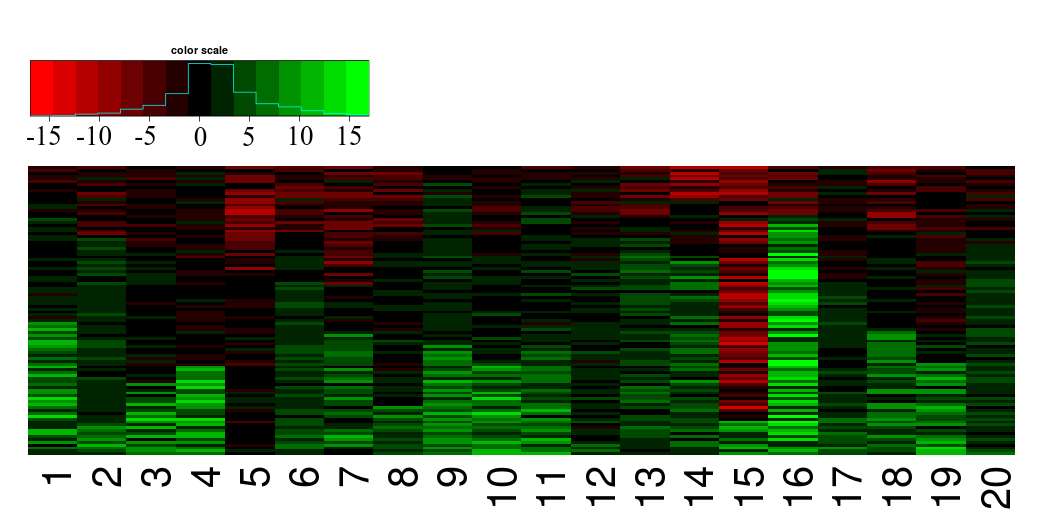
\includegraphics[scale = 0.3]{./veera/true_y_heatmap_sim_final.png}
        \caption{Simulated $y_{sg}$ ordered by true $e_{sg}$.}
        \vspace{0.5 cm}
    \end{subfigure}\\
    ~
    \begin{subfigure}[b]{0.98\textwidth}
        \centering
        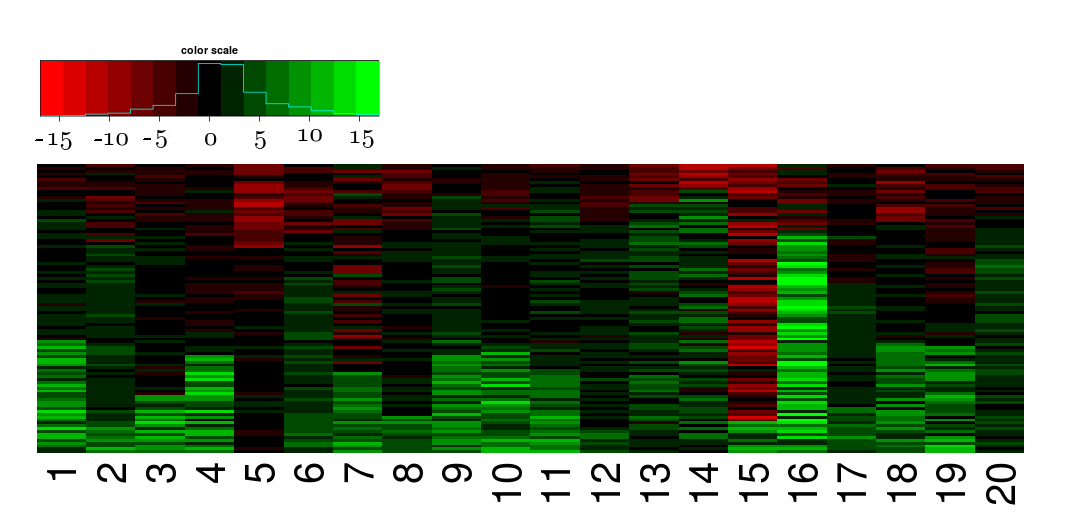
\includegraphics[scale = 0.3]{./veera/estimated_y_heatmap_sim_final.png}
        \caption{Simulated $y_{sg}$ ordered by estimated $e_{sg}$.}
        \vspace{0.5 cm}
    \end{subfigure}\\
    ~ 
    \begin{subfigure}[b]{0.98\textwidth}
        \centering
        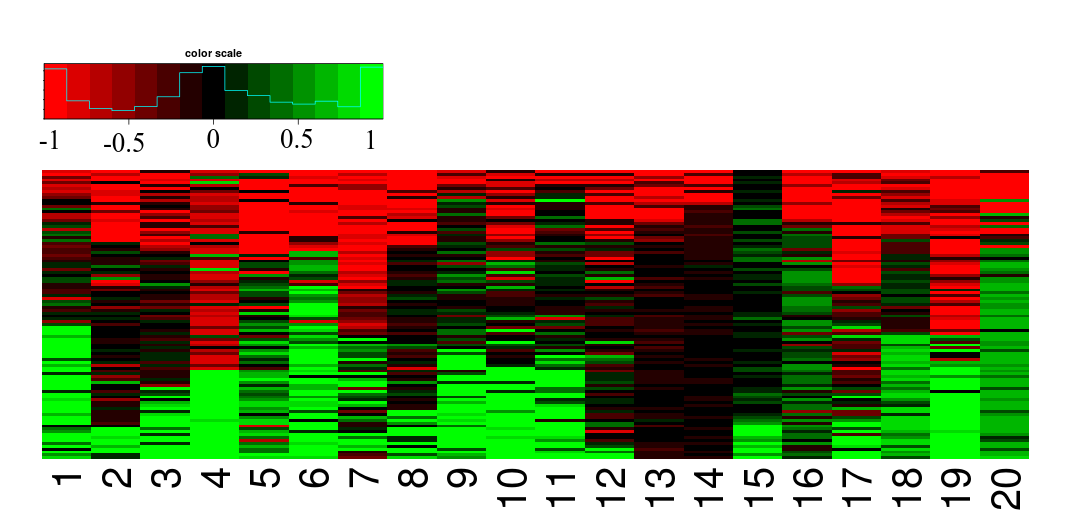
\includegraphics[scale = 0.3]{./veera/estimated_d_heatmap_sim_final.png}
        \caption{$d_{sg}$ ordered by true $e_{sg}$.}
	\vspace{0.5 cm}
    \end{subfigure}
    \caption{(a): Simulated data $y_{sg}$. Samples in each column are sorted by true $e_{sg}$. (b) Simulated data $y_{sg}$. Samples in each column are sorted by estimated $E\left( e_{sg} \mid \bfy \right)$. (c) Differences $d_{sg}=p^+_{sg} - p^-_{sg}$ with the same ordering as in panel (a). The ordering of samples change according to the protein (column) but is the same throughout the 3 panels.}
\label{fig:sim_poe_heatmap_1}
\end{figure}


%\begin{figure}[H]
%    \centering
%    \begin{subfigure}[b]{0.54\textwidth}
%        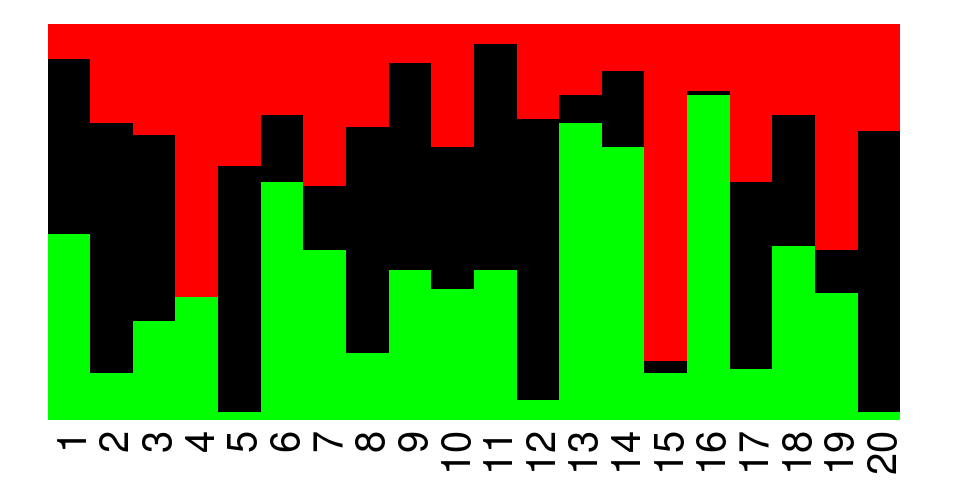
\includegraphics[scale = 0.25]{./veera/true_e_heatmap_sim.png}
%        \caption{Simulated $e_{sg}$.}
%    \end{subfigure}%
%    ~
%    \begin{subfigure}[b]{0.54\textwidth}
%        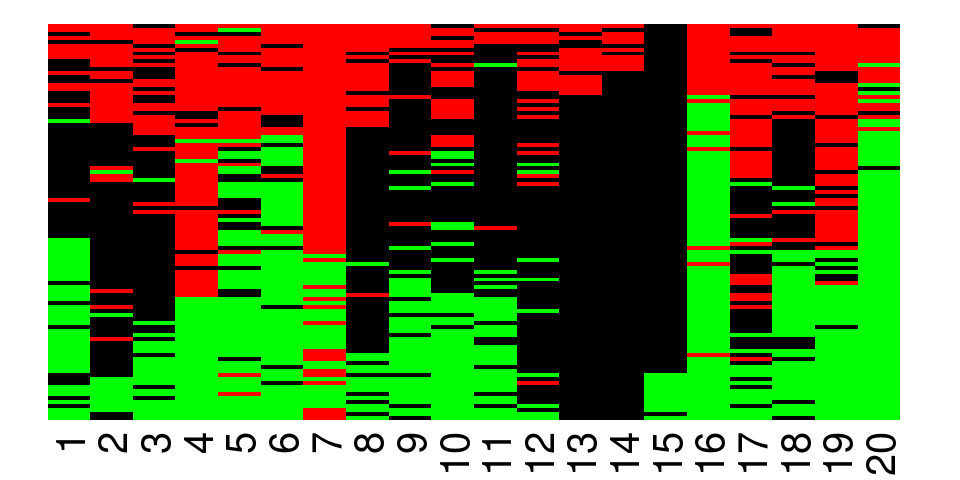
\includegraphics[scale = 0.25]{./veera/estimated_e_heatmap_sim.png}
%        \caption{Estimated $e_{sg}$.}
%    \end{subfigure}
%    \caption{(a) Simulation truth: $e_{sg}=1$ (green), $e_{sg}=0$ (black), $e_{sg}=-1$ (red).  (b) Point estimates of $e_{sg}$. Rows represent tumors (samples) while columns represent genes (proteins). Each column is ordered in a different way within each heatmap. The ordering of samples change according to the protein (column) but is the same throughout the 2 panels.}
%\label{fig:sim_poe_heatmap_2}
%\end{figure}


%\begin{figure}[H]
%\centering
%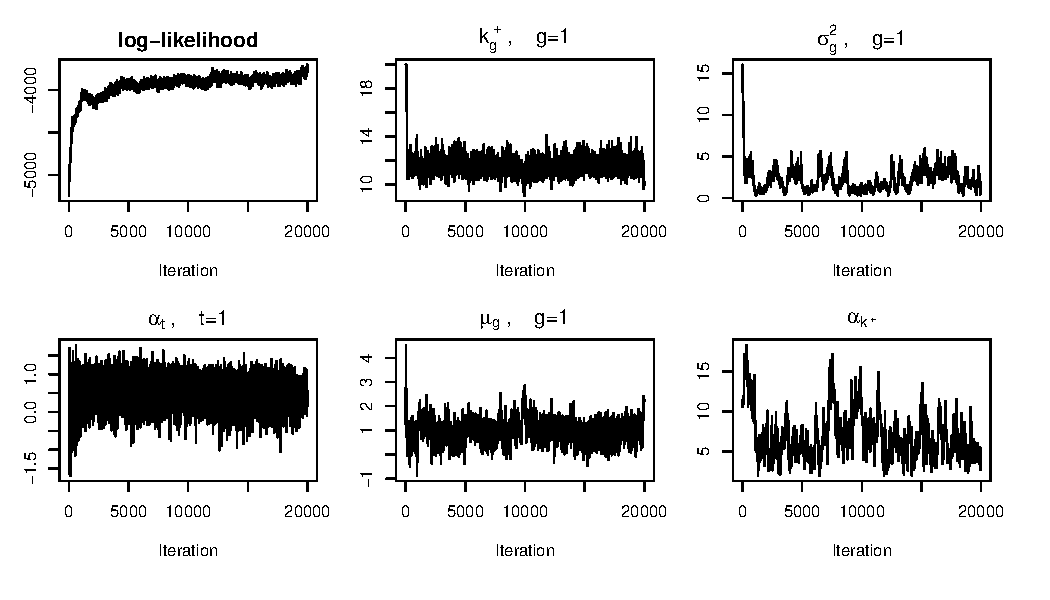
\includegraphics[scale=0.75]{./veera/mcmc_chains_sim.pdf}
%\caption{MCMC samples for the log-likelihood and for some of the marginals.}
%\label{fig:traces_poe}
%\end{figure} 

\begin{figure}[H]
\centering
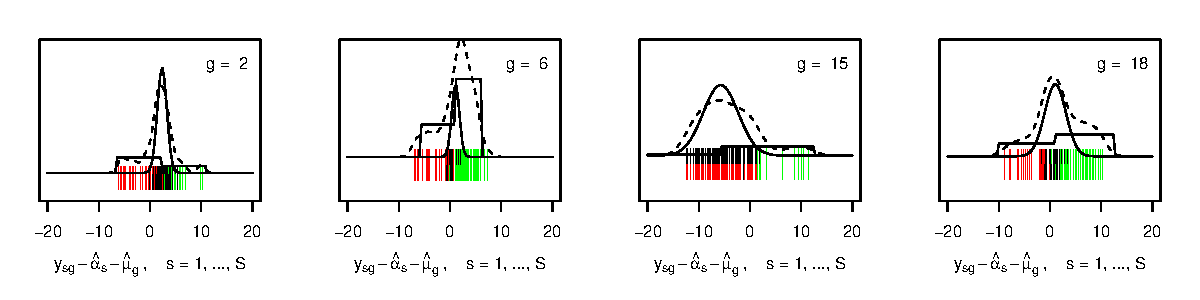
\includegraphics[scale=0.7]{./veera/density_estimates_sim_subset.pdf}
\caption{Posterior density estimates. Vertical bars represent centralized gene expressions $y_{sg} - \mu_g - \alpha_s, \ s = 1, ..., S$ for all genes $g$ collored according to its estimated cluster membersip indicators (top) and true cluster membership indicators (bottom). Full lines represent the best fitting uniform and normal components of the mixture a posteriori multiplied by the respective weights. Dashed line corresponds to a kernel density estimate based on the vertical bars. Color code: black = -1, red = 0, green = 1.}
\label{fig:poe_densities}
\end{figure} 


\subsection{Simulation 2: nested partitions}

In this section we describe the simulation to validate inference on the NobLoc model. We replicated the scenario in \cite{lee2013}, with 100 samples and 20 proteins. The simulation truth incorporates the local clustering feature of first partitioning proteins and then within protein cluster, partitioning the samples. However, instead of simulating the protein and sample partitions according to a zero inflated Pólya urn, we fixed the partition of proteins upfront to have two active protein clusters, the first one containing  proteins with 3 active sample clusters; and the second containing 4 proteins with 2 active sample clusters. The cluster-membership assignment of samples was made uniformly at random among the available sample clusters. The cluster specific means were fixed at the same values in Table 1 of \cite{lee2013}. Inactive samples and proteins were all sampled from $Unif(-0.8, 0.8)$. The standard deviation of the Gaussian sampling model for active samples was fixed at $\sigma_g = 0.1$ For an illustration, see Figure \ref{fig:nobloc_sim_fit} panel (a). 

In Figure \ref{fig:nobloc_sim_fit} panel (b) we can see that the underlying cluster structure was reasonably captured by the NobLoc model. The only discrepancy is the inclusion of protein 19 in the first active cluster together with proteins 1 - 8, instead of classifying it as an inactive protein according to the simulation truth.

\begin{figure}[H]
\centering
\begin{subfigure}[b]{0.48\textwidth}
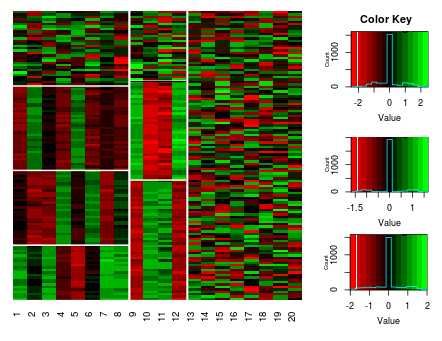
\includegraphics[scale=0.5]{./veera/true_heatmap_nobloc_sim.png} %\hspace{1cm}
\caption{Simulated $y_{sg}$ ordered by \\ true cluster assignments.}
\end{subfigure}
\begin{subfigure}[b]{0.48\textwidth}
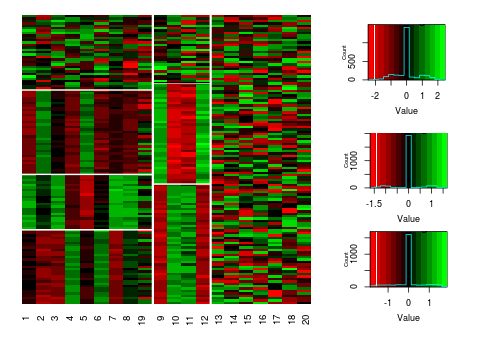
\includegraphics[scale=0.5]{./veera/mcmc_heatmap_nobloc_sim.png}
\caption{Simulated $y_{sg}$ ordered by \\ estimated cluster assignments.}
%\vspace{0.5 cm}
\end{subfigure}
\caption{(a): Observations ordered according to the simulation truth. (b): Observations ordered according to estimated cluster membership indicators a posteriori. In both panels, rows represent samples while columns represent proteins.}
\label{fig:nobloc_sim_fit}
\end{figure} 


\section{Lung Cancer Dataset}

\subsection{The data}

The dataset consists of protein profiles coming from an RPPA experiment on lung cancer samples. The data records 233 proteins  that were pre-selected for their biological relevance to the study of this type of cancer. The data records samples from 687 patients and 124 cell lines. The objective is to identify groups of similar patients and cell lines with respect to subgroups of co-expressed proteins (we informaly say that proteins are co-expressed if their expressions are correlated). We therefore expect that the samples (patients and cell lines) can be partitioned in a different way depending on the group of co-expressed proteins that is considered. 

\subsection{Results}

We describe here the results of a joint inference of the POE model and nested clustering by NoB-LoC. We start by analyzing the results of directly applying the NoB-LC model to the original lung data (without running POE first), which is illustrated in Figure \ref{fig:nobloc_fit} (a).

\begin{figure}[H]
\centering
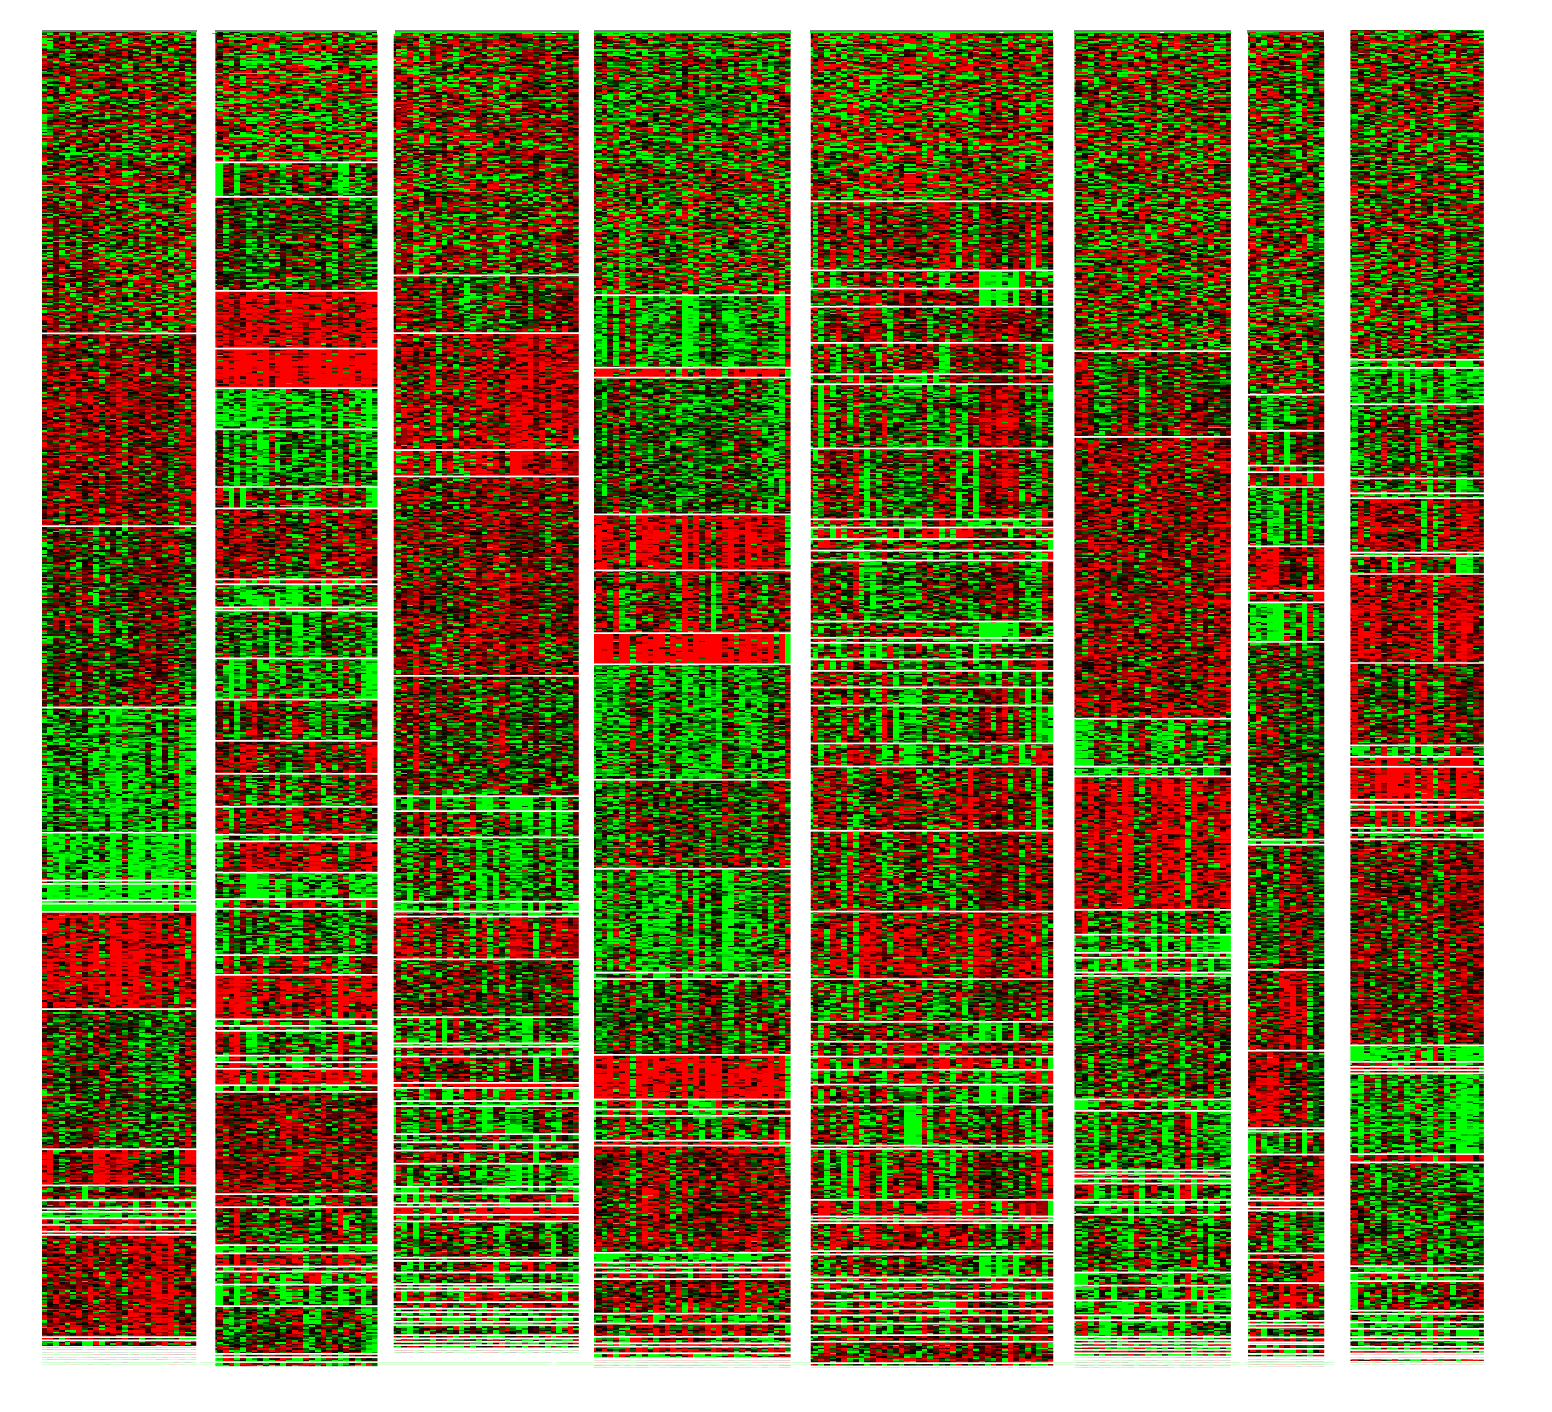
\includegraphics[scale=0.12]{./veera/all_heatmap_no_poe.png} \hspace{2cm}
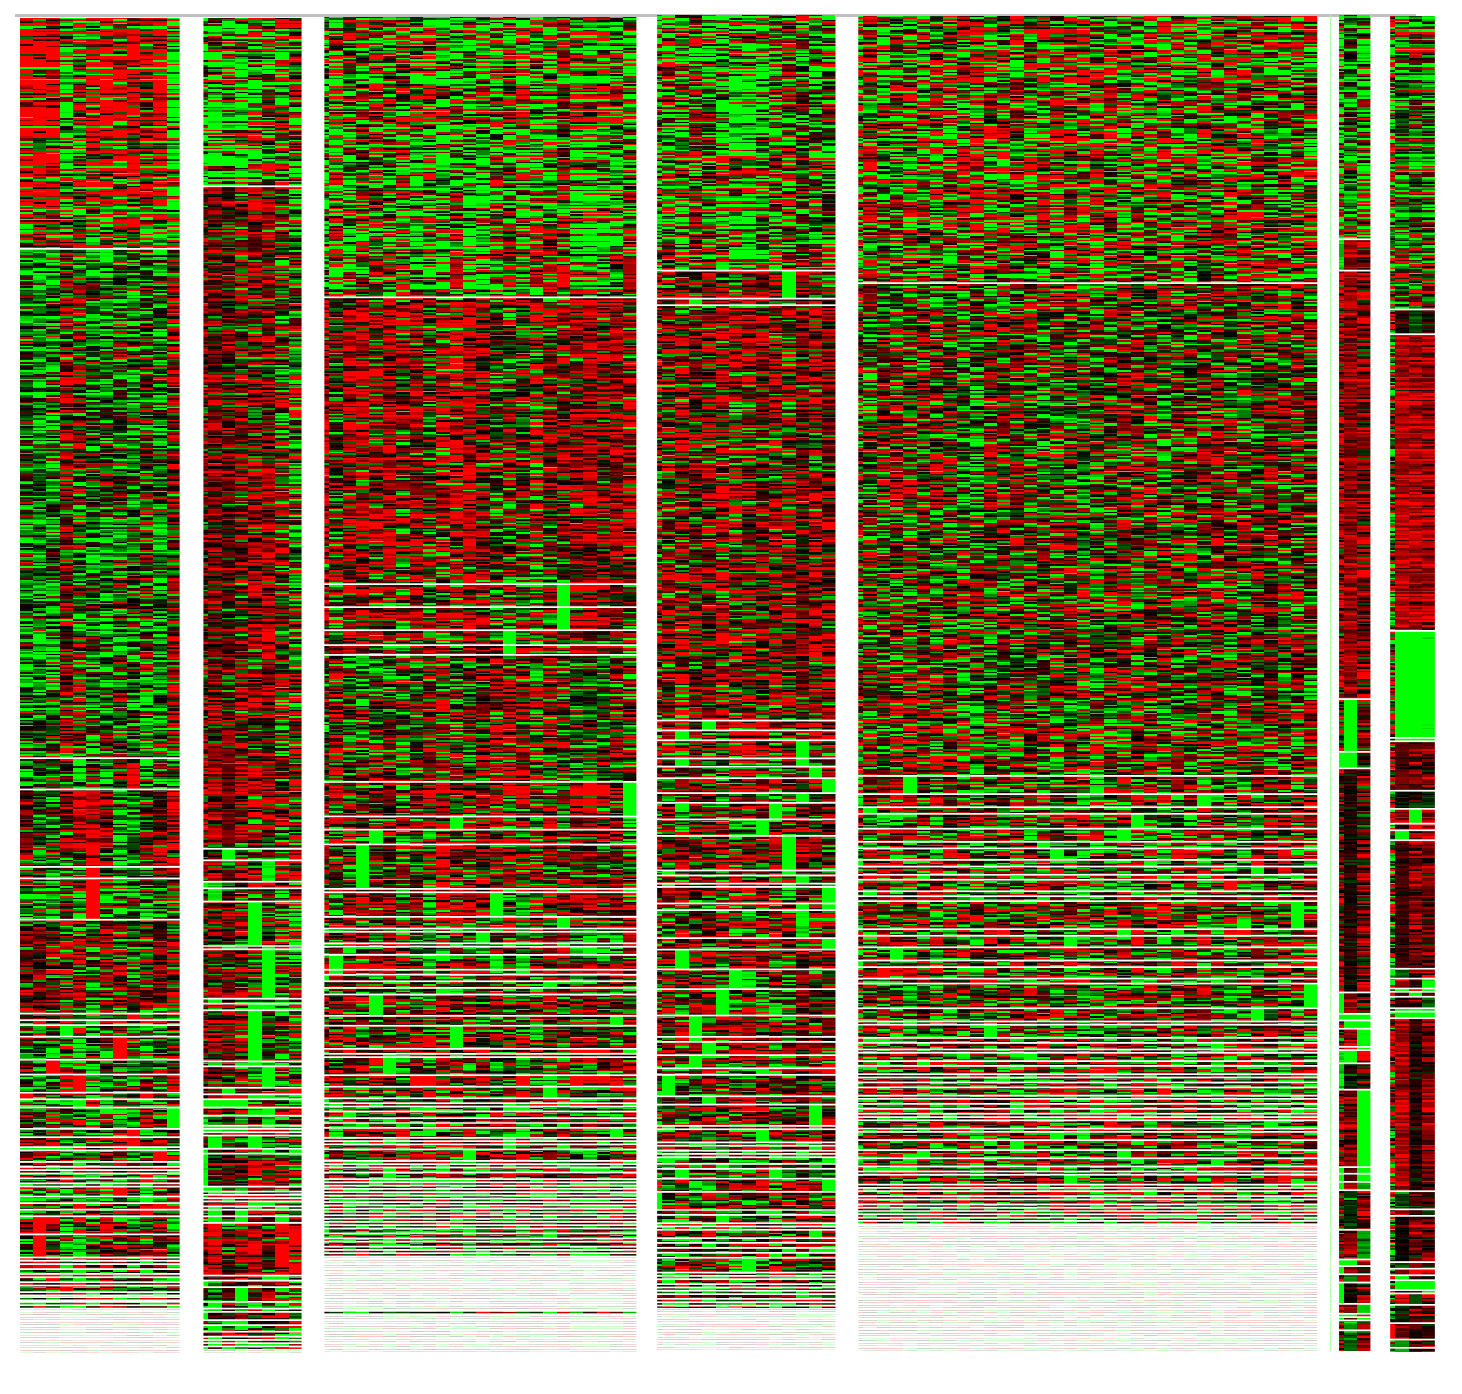
\includegraphics[scale=0.12]{./veera/all_heatmap_after_poe.png}
\caption{Observed protein expression arranged according to posterior estimated cluster structure under NoB-Loc. Only active proteins are displayed. Panel (a) shows the result of application of the NobLoc model on the original data and panel (b) shows the results after the application of POE.}
\label{fig:nobloc_fit}
\end{figure} 

Figure \ref{fig:match_patients_cell_lines} shows one of the blocks in Figure \ref{fig:nobloc_fit} in more details highlighting the similarities between the cell lines and proteins in that block. Samples are reasonably homogeneous in terms of the expressions of the particular subgroup of proteins shown in the figure. Notice also that some proteins present typically high expression while others typically present low expression considering the particular group of samples.


\begin{figure}[H]
\centering
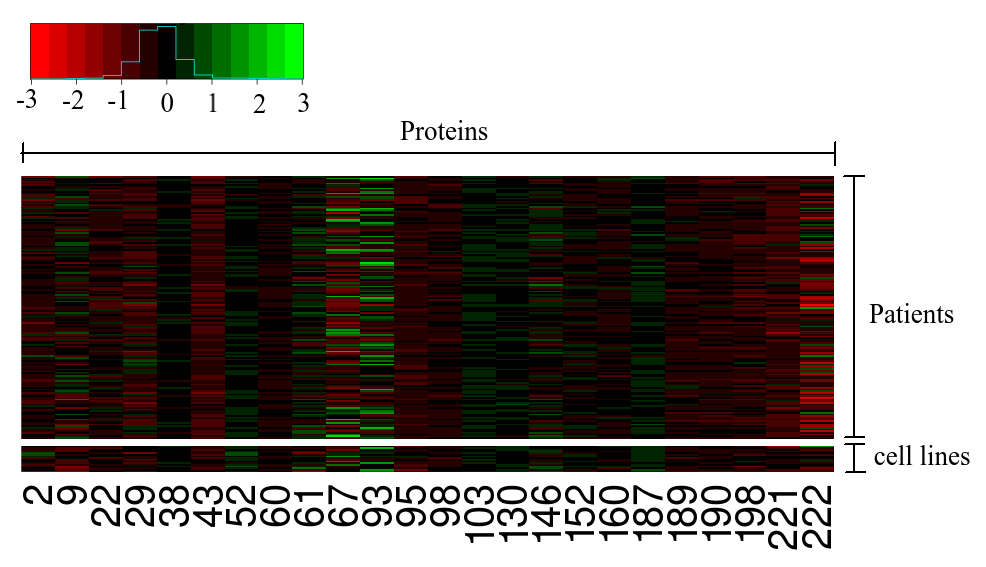
\includegraphics[scale=0.5]{./veera/zoom_after_poe_new.png}
\caption{Protein expressions within one of the samples/proteins blocks of Figure \ref{fig:nobloc_fit} (b). The cell lines and patients exhibit very similar profiles when considering the subset of proteins that were clustered together by the model.}
\label{fig:match_patients_cell_lines}
\end{figure} 

\section{Discussion and Future Directions}

Some innovations were introduced in this chapter: (i) The model naturally accounts for co-expression of genes and/or proteins in a manner that allows distinct clustering of samples depending on each estimated subgroup of co-expressed functional units or pathways; (ii) We develop efficient models for “matching” patients and cell line profiles. Development of such inferential tools is of critical relevance to implementing precision medicine, since it can be used for potential treatment assignment that is specific to a patient, and borrows information not only from that patient, but also from cell lines coming from external sources. The latter is critical also because experiments with cell lines can be carried out freely. (iii) Third, the approach does not need to be restricted to cell lines and patients but can be generalized to multiplatform omics profiles from diverse model systems such as patient-derived xenographs (PDX) models and organoids.

This chapter makes two important methodological contributions in Bayesian non-parametrics: (i) the seamless integration of the (modified) probability of expression (POE) model for noise reduction and the nested bi-clustering approach; (ii) the formal probabilistic modeling of co-clustering between cell lines and patients based on profile similarities via dependent priors on partition models.

There are some areas that need to be more thoroughly investigated. One of them is the need to extend the simulation studies where the underlying truth differs from the POE and NobLoc models in order to address the performance of the proposed methodology under model misspecification. In our results, we restricted the matching of cell lines and patients to a conditional zero inflated P\'olya urn (see section \ref{sec:nobloc_matching}), therefore the investigation of the other models for matching information from cell lines to patients is also proposed as a future work.

One of the limitations of the oroposed approach is the computational effort of full posterior simulation. Alternative implementations based on variational inference for example are possible alternatives (see section 1.4).